\ifx\wholebook\relax \else
\documentclass[b5paper]{ctexart}
\usepackage[nomarginpar
  %, margin=.5in
]{geometry}

\addtolength{\oddsidemargin}{-0.05in}
\addtolength{\evensidemargin}{-0.05in}
\addtolength{\textwidth}{0.1in}
\usepackage[cn]{../../../prelude}

\setcounter{page}{1}

\begin{document}

\title{序列}

\author{刘新宇
\thanks{{\bfseries 刘新宇 } \newline
  Email: liuxinyu95@gmail.com \newline}
  }

\maketitle
\fi

\markboth{序列}{基本算法}

\ifx\wholebook\relax
\chapter{序列}
\numberwithin{Exercise}{chapter}
\fi

\section{简介}
\label{introduction}

序列是对数组和列表的一种抽象组合。我们希望理想的序列能达到下面的要求:

\begin{enumerate}
\item 可以在头部、尾部以常数时间插入、删除元素;
\item 可以快速(优于线性时间)连接两个序列;
\item 可以快速随机访问、更改任何元素;
\item 可以快速在指定位置断开序列。
\end{enumerate}

数组、列表仅部分满足这些要求,如下表所示。其中$n$为单个序列的长度,$n_1$、$n_2$分别表示被连接的两个序列的长度。

\btab{| l | c | r |}
  \hline
  操作 & 数组 & 列表 \\
  \hline
  在头部插入、删除 & $O(n)$ & $O(1)$ \\
  在尾部插入、删除 & $O(1)$ & $O(n)$ \\
  连接 & $O(n_2)$ & $O(n_1)$ \\
  随机访问位置$i$ & $O(1)$ & $O(i)$ \\
  在位置$i$删除 & $O(n-i)$ & $O(1)$ \\
  \hline
\etab

本章我们给出三种序列实现:二叉随机访问列表、可连接列表、手指树。

\section{二叉随机访问列表}
\index{序列!二叉随机访问列表}

二叉随机访问列表是由二叉树森林实现的随机访问列表。森林包含若干完全二叉树。元素只保存在叶子节点中。对任何非负整数$n$,将其表达为二进制,我们就知道需要多少棵完全二叉树来存储$n$个元素。每个值为1的二进制位代表一棵二叉树,树的大小对应着二进制位的高低。任给索引$1 \leq i \leq n$,我们都可以快速在森林中定位到保存第$i$个节点的二叉树。如图\ref{fig:bi-tree-sequence}所示,树$t_1$、$t_2$表示序列$[x_1, x_2, x_3, x_4, x_5, x_6]$。

\begin{figure}[htbp]
  \centering
  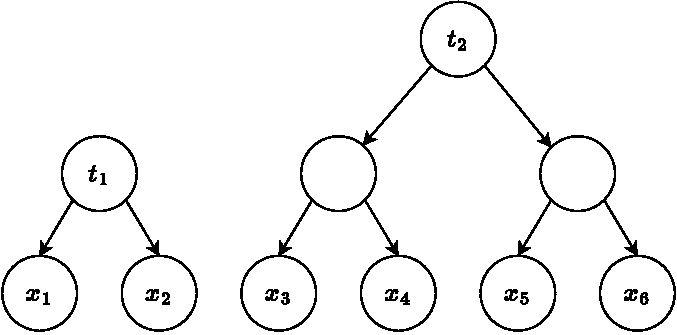
\includegraphics[scale=0.5]{img/bi-tree-sequence}
  \caption{含有6个元素的序列}
  \label{fig:bi-tree-sequence}
\end{figure}

记深度为$i+1$的完全二叉树为$t_i$。$t_0$只含有一个叶子节点。$t_i$含有$2^i$个叶子。对于$n$个元素的序列,我们把$n$表示为二进制数$n = (e_m e_{m-1} ... e_1 e_0)_2$,其中$e_i$为1或0。

\be
n = 2^0 e_0 + 2^1 e_1 + ... + 2^m e_m
\ee

如果$e_i \neq 0$,就需要一棵大小为$2^i$的完全二叉树$t_i$。在图\ref{fig:bi-tree-sequence}的例子中,序列长度为$6 = (110)_2$。最低位是0,我们不需要大小为1的树;第2位是1,需要一棵大小为2的树$t_1$;最高位是1,需要一棵大小为4的树$t_2$。这样就把序列$[x_1, x_2, ..., x_n]$表示为树的列表。列表中每棵树的大小都是唯一的,并按照从小到大排列。我们称之为\textbf{二叉随机访问列表}\cite{okasaki-book}。我们可以在二叉树定义的基础上稍作变化以实现这种列表:1、元素只保存在叶子节点中,2、在每棵子树中记录树的大小。这样每个分枝节点记为$(s, l, r)$,其中$s$表示子树的大小,$l$、$r$分别表示左右子树。包含元素$x$的叶子节点记为$(x)$。我们可以这样获取一棵树的大小:

\be
\begin{array}{rcl}
size\ (x) & = & 1 \\
size\ (s, l, r) & = & s \\
\end{array}
\ee

\index{二叉随机访问列表!插入}
为了把新元素$y$插入到序列$S$的前面,我们创建一棵只有一个叶子节点的$t_0$树:$t' = (y)$,然后把它插入到森林中。$insert\ y\ S = insert_T\ (y)\ S$,或写成克里化形式:

\be
insert\ y = insert_T\ (y)
\ee

我们检查森林中的第一棵树$t_i$,比较$t_i$和$t'$的大小,如果$t_i$较大,就将$t'$置于森林最前面(常数时间);若$t_i$和$t'$相等,我们将它们链接(常数时间)成一棵较大的树:$t'_{i+1} = (2s, t_i, t')$,然后递归地将$t'_{i+1}$插入到森林中。如图\ref{fig:bralist-2}所示。

\be
\begin{array}{rcl}
insert_T\ t\ [\ ] & = & [t] \\
insert_T\ t\ (t_1 \cons ts) & = & \begin{cases}
  size\ t < size\ t_1: & t : t_1 : ts \\
  \text{否则}: & insert_T\ (link\ t\ t_1)\ ts \\
  \end{cases}
\end{array}
\ee

其中$link$将两棵大小相同的树链接起来:$link\ t_1\ t_2 = (size\ t_1 + size\ t_2, t_1, t_2)$。

\begin{figure}[htbp]
  \centering
  \subcaptionbox{插入$x_1$。}{\hspace{0.2\textwidth}\includegraphics[scale=0.5]{img/bralst-1}\hspace{0.2\textwidth}}
  \subcaptionbox{插入$x_2$,链接产生$[t_1]$。}{\hspace{0.2\textwidth}\includegraphics[scale=0.5]{img/bralst-2}\hspace{0.2\textwidth}} \\
  \subcaptionbox{插入$x_3$,结果为$[t_0, t_1]$。}{\hspace{0.2\textwidth}\includegraphics[scale=0.5]{img/bralst-3}\hspace{0.2\textwidth}}
  \subcaptionbox{插入$x_4$。经两次链接后结果为$[t_2]$。}{\includegraphics[scale=0.5]{img/bralst-4}} \\
  \subcaptionbox{插入$x_5$,结果为:$[t_0, t_2]$。}{\includegraphics[scale=0.5]{img/bralst-5}}
  \subcaptionbox{插入$x_6$,结果为:$[t_1, t_2]$。}{\hspace{0.1\textwidth}\includegraphics[scale=0.5]{img/bralst-6}} \\
  \caption{插入$x_1, x_2, ..., x_6$}
  \label{fig:bralist-2}
\end{figure}

若森林中包含$m$棵树,$m$的大小为$O(\lg n)$,头部插入的性能为$O(\lg n)$。稍后我们证明分摊性能为常数时间。

\index{二叉随机访问列表!从头部删除}
对称地,我们利用插入的逆过程实现从序列头部删除元素。如果森林中第一棵树是$t_0$(单叶子节点),我们直接将$t_0$删除;否则,递归地将第一棵树拆分直到获得$t_0$,然后将其删除。如图\ref{fig:bralist-pop}所示。

\begin{figure}[htbp]
  \centering
  \subcaptionbox{序列$x_1, x_2, ..., x_5$对应森林$[t_0, t_2]$}{\includegraphics[scale=0.5]{img/bralst-5}}
  \subcaptionbox{删除$x_5$。直接删除$t_0$。}{\includegraphics[scale=0.5]{img/bralst-4}} \\
  \subcaptionbox{删除$x_4$。经过两次拆分后得到$[t_0, t_0, t_1]$,删除后得$[t_0, t_1]$。}{\hspace{0.2\textwidth}\includegraphics[scale=0.5]{img/bralst-3}\hspace{0.2\textwidth}}
  \caption{从头部删除元素}
  \label{fig:bralist-pop}
\end{figure}

\be
\begin{array}{rcl}
extract\ ((x) \cons ts) & = & (x, ts) \\
extract\ ((s, t_1, t_2) \cons ts) & = & extract\ (t_1 \cons t_2 \cons ts) \\
\end{array}
\ee

利用$extract$即可实现对头部元素的删除:

\be
\begin{cases}
head & = \textit{fst} \circ extract \\
tail & = \textit{snd} \circ extract \\
\end{cases}
\ee

其中$\textit{fst}\ (a, b) = a$, $\textit{snd}\ (a, b) = b$分别返回一对值中的两个部分。

\index{二叉随机访问列表!随机访问}
森林中的树实际上将元素划分为大小不同的区块。给定任意索引$1 \leq i \leq n$,我们先定位到对应的完全二叉树,然后再进行一次树查找就可定位到元素。

\begin{enumerate}
\item 比较$i$和森林中第一棵树$t$的大小,若$i \leq size(t)$,则元素在$t$中,接下来在树$t$中进行查找;
\item 否则,令$i' = i - size(t)$,然后递归地在剩余的树中查找第$i'$个元素。
\end{enumerate}

\be
(t \cons ts)[i] = \begin{cases}
  i \leq size\ t: & lookup_T\ i\ t \\
  \text{否则}: & ts[i - size\ t] \\
\end{cases}
\ee

其中$lookup_T$在树中进行二分查找。如果$i = 1$,我们返回根节点;否则,我们将树拆半,然后递归查找:

\be
\begin{array}{rcl}
lookup_T\ 1\ (x) & = & x \\
lookup_T\ i\ (s, t_1, t_2) & = & \begin{cases}
  i \leq \lfloor \dfrac{s}{2} \rfloor: & lookup_T\ i\ t_1 \\
  \text{否则}: & lookup_T\ (i - \lfloor \dfrac{s}{2} \rfloor)\ t_2 \\
  \end{cases}
\end{array}
\ee

图\ref{fig:get-at-example}描述了在一个长度为6的序列中查找第4个元素的步骤。第一棵树大小为2 < 4,继续检查第二棵树,并将索引更新为$i' = 4 - 2 $。接下来的树大小为$4 > i' = 2$,故待查找元素就在这棵树中。因为索引为2,不大于拆半的子树大小$4/2 = 2$,所以接下来检查左子树,然后检查右侧的孙子分支,最终得到要访问的元素。类似地,我们也可以修改任意位置$i$的元素。

\begin{figure}[htbp]
  \centering
  \subcaptionbox{$S[4], 4 > size(t_1) = 2$}{\includegraphics[scale=0.5]{img/bralst-6}}
  \subcaptionbox{$S'[4-2] \Rightarrow lookup_T\ 2\ t_2$}{\hspace{0.2\textwidth}\includegraphics[scale=0.5]{img/bralst-4}\hspace{0.2\textwidth}} \\
  \subcaptionbox{$ 2 \leq \lfloor \dfrac{size(t_2)}{2} \rfloor \Rightarrow lookup_T\ 2\ left(t_2)$}{\hspace{0.2\textwidth}\includegraphics[scale=0.5]{img/bralst-4l}\hspace{0.2\textwidth}}
  \subcaptionbox{$lookup_T\ 1\ right(left(t_2))$, 返回$x_3$}{\hspace{0.2\textwidth}\includegraphics[scale=0.5]{img/bralst-4lr}\hspace{0.2\textwidth}}
  \caption{获取$S[4]$}
  \label{fig:get-at-example}
\end{figure}

根据完全二叉树的性质,对于含有$n$个元素的序列,树木的棵数为$O(\lg n)$。对于索引$i$,最多需要$O(\lg n)$时间来定位到树。接下来的搜索和树的高度成正比,最多也是$O(\lg n)$。因此随机访问的总体性能为$O(\lg n)$。

\begin{Exercise}
如何处理索引越界情况?
\end{Exercise}

\section{数字表示}
\index{序列!二叉随机访问列表的数字表示}

非负整数$n$的二进制形式和森林之间存在关系:$n = 2^0e_0 + 2^1e_1 + ... + 2^me_m$,其中$e_i$为第$i$位的值。若$e_i = 1$,则存在一棵大小为$2^i$的完全二叉树。向序列头部插入元素,对应于二进制数加1;而删除对应二进制数减1。我们称这种关系为\underline{数字表示}\cite{okasaki-book}。为了明确表示这种对应,我们为每个二进制位定义两个状态:状态零$Zero$表示不存在二叉树,而状态一$One\ t$表示存在二叉树$t$。这样森林就可以表示为一组二进制状态的列表,从而把插入实现为二进制数的增加。

\be
\begin{array}{rcl}
add\ t\ [\ ] & = & [One\ t] \\
add\ t\ (Zero \cons ds) & = & (One\ t) : ds \\
add\ t\ (One\ t' \cons ds) & = & Zero : add\ (link\ t\ t')\ ds
\end{array}
\ee

将树$t$插入森林对应二进制加法:若森林为空,我们创建状态$One\ t$,它是二进制数中的唯一位。相当于$0 + 1 = 1$。若森林不空,如果二进制首位数字是$Zero$,我们创建一个状态$One\ t$替换掉$Zero$。这相当于二进制加法$(...digits...0)_2 + 1 = (...digits...1)_2$。例如$6 + 1 = (110)_2 + 1 = (111)_2 = 7$。如果二进制首位是$One\ t'$,我们认为$t$和$t'$的大小相同。这是因为我们总是以一个叶子$t_0 = (x)$开始插入,待插入树的大小逐渐增长,呈一个序列$1, 2, 4, ..., 2^i, ...$。我们将$t$和$t'$链接起来,递归地插入到剩余的数字中。而之前的$One\ t'$被替换为$Zero$。这相当于二进制加法$(...digits...1)_2 + 1 = (...digits'...0)_2$。例如$7 + 1 = (111)_2 + 1 = (1000)_2 = 8$。

接下来我们用二进制减法来表示删除。如果序列只含有一位$One\ t$,删除后序列变为空。这对应二进制减法$1 - 1 = 0$。如果序列有多位,并且首位是$One\ t$,我们将其替换为$Zero$。这相当于二进制减法 $(...digits...1)_2 - 1 = (...digits...0)_2$。例如$7 - 1 = (111)_2 - 1 = (110)_2 = 6$。如果首位是$Zero$,减法需要借位。我们递归地从剩余的数字中抽取树,将其分拆成两棵树$t_1$、$t_2$,将$Zero$替换成$One\ t_2$,并删除$t_1$。这相当于二进制减法$(...digits...0)_2 - 1 = (...digits'...1)_2$。例如$4 - 1 = (100)_2 - 1 = (11)_2 = 3$。

\be
\begin{array}{rcl}
minus\ [One\ t] & = & (t, [\ ]) \\
minus\ ((One\ t) \cons ts) & = & (t, Zero \cons ts) \\
minus\ (Zero \cons ts) & = & (t_1, (One\ t_2) \cons ts'), \text{其中}: (s, t_1, t_2) = minus\ ts \\
\end{array}
\ee

数字表示并没有改变复杂度。我们使用聚合方法法,分析在插入的分摊复杂度。考虑依次向空序列插入$n = 2^m$个元素的过程。森林的二进制表示如表\ref{tab:ralist-insertion}:

\begin{table}[htbp]
\centering
\begin{tabular}{|l|r|}
  \hline
  i & 二进制(高 ... 低) \\
  \hline
  0 & 0, 0, ..., 0, 0 \\
  1 & 0, 0, ..., 0, 1 \\
  2 & 0, 0, ..., 1, 0 \\
  3 & 0, 0, ..., 1, 1 \\
  ... & ... \\
  $2^m-1$ & 1, 1, ..., 1, 1 \\
  $2^m$ & 1, 0, 0, ..., 0, 0 \\
  \hline
  位变化次数 & 1, 1, 2, ... $2^{m-1}$, $2^m$ \\
  \hline
\end{tabular}
\caption{插入$2^m$个元素的过程}
\label{tab:ralist-insertion}
\end{table}

二进制表示的最低位每次插入时都变化,总共需要$2^m$次计算;次低位每隔一次变化,执行一次树的链接操作。共需要$2^{m-1}$次计算;次高位总共只变化一次,将所有的树链接成一棵大树。最后一个元素插入后,最高位变为1。将所有计算次数相加,得到$T = 1 + 1 + 2 + 4 + ... + 2^{m-1} + 2^m = 2^{m+1}$。平均每次插入操作的分摊复杂度为:

\be
O(T/n) = O(\dfrac{2^{m+1}}{2^m}) = O(1)
\ee

这就证明了插入的分摊复杂度为常数时间。

\begin{Exercise}
\Question{实现数值表示序列的随机访问$S[i], 1 \leq i \leq n$。其中$n$是序列长度。}
\Question{使用聚合法,证明删除的分摊复杂度为常数时间。}
\Question{可以用长度为$2^m$的数组表示完全二叉树($m$是非负整数)。请用数组实现二叉树森林的插入和随机访问。并分析它们的分摊复杂度。}
\end{Exercise}

\section{双数组序列}
\index{序列!双数组序列} \index{双数组列表!插入和添加}

在上一章中,我们给出过双数组队列。由于数组可以常数时间随机访问,我们可以将其扩展为双数组序列。如图\ref{fig:parrays},按头对头的方式连接两个数组。在列表的头部插入时,添加到$f$数组末尾;向尾部插入时,添加到$r$数组末尾。这样我们用一对数组表示列表$S = (f, r)$,令$\textproc{Front}(S) = f$,$\textproc{Rear}(S) = r$。前后插入实现如下:

\begin{figure}[htbp]
  \centering
  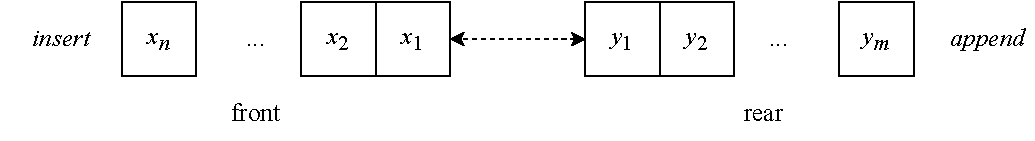
\includegraphics[scale=0.7]{img/parrays}
  \caption{双数组序列}
  \label{fig:parrays}
\end{figure}

\begin{algorithmic}[1]
\Function{Insert}{$x, S$}
  \State \textproc{Append}($x$, \Call{Front}{$S$})
\EndFunction
%\Statex
\Function{Append}{$x, S$}
  \State \textproc{Append}($x$, \Call{Rear}{$S$})
\EndFunction
\end{algorithmic}

\index{双数组列表!随机访问}
随机访问第$i$个元素时,我们先判断$i$索引到$f$还是$r$,然后再定位到元素。若$ i \leq |f|$,元素在$f$中。由于$f$和$r$头对头连接的,所以$f$按照从右向左逆序索引元素。我们用$|f| - i + 1$定位到元素;如果$i > |f|$,元素在$r$中。元素是从左向右索引的,我们用$i - |f|$定位到元素。

\begin{algorithmic}[1]
\Function{Get}{$i, S$}
  \State $f, r \gets $ \Call{Front}{$S$}, \Call{Rear}{$S$}
  \State $n \gets $ \Call{Size}{$f$}
  \If{$i \leq n $}
    \State \Return $f[n - i + 1]$ \Comment{反向索引}
  \Else
    \State \Return $r[i - n]$
  \EndIf
\EndFunction
\end{algorithmic}

\index{双数组列表!删除和平衡}
删除可能把一个数组$f$或$r$变空,而另一个仍有元素,需要恢复平衡。当$f$或$r$等于$[\ ]$时,我们将另一数组分成两半,然后将前一半反转形成一对新的数组。$f$、$r$是对称的。我们也可以交换$f$、$r$,递归调用\textproc{Balance},再把$f$、$r$交换回来。

\begin{algorithmic}[1]
\Function{Balance}{$S$}
  \State $f \gets$ \Call{Front}{$S$}, $r \gets$ \Call{Rear}{$S$}
  \State $n \gets$ \Call{Size}{$f$}, $m \gets$ \Call{Size}{$r$}
  \If{$F = [\ ]$}
    \State $k \gets \lfloor \dfrac{m}{2} \rfloor$
    \State \Return $(\textproc{Reverse}(r[1 ... k]), r[(k + 1) ... m])$
  \EndIf
  \If{$R = [\ ]$}
    \State $k \gets \lfloor \dfrac{n}{2} \rfloor$
    \State \Return $(f[(k + 1) ... n], \textproc{Reverse}(f[1 ... k]))$
  \EndIf
  \State \Return $(f, r)$
\EndFunction
\end{algorithmic}

在每次删除时,我们都检查$f$、$r$是否为空,并触发平衡操作:

\begin{algorithmic}[1]
\Function{Remove-Head}{$S$}
  \State \Call{Balance}{$S$}
  \State $f, r \gets$ \Call{Front}{$S$}, \Call{Rear}{$S$}
  \If{$f = [\ ]$} \Comment{$S = ([], [x])$}
    \State $r \gets [\ ]$
  \Else
    \State \Call{Remove-Last}{$f$}
  \EndIf
\EndFunction
\Statex
\Function{Remove-Tail}{$S$}
  \State \Call{Balance}{$S$}
  \State $f, r \gets$ \Call{Front}{$S$}, \Call{Rear}{$S$}
  \If{$r = [\ ]$} \Comment{$S = ([x], [])$}
    \State $f \gets [\ ]$
  \Else
    \State \Call{Remove-Last}{$r$}
  \EndIf
\EndFunction
\end{algorithmic}

由于要进行反转,双数组序列在最坏情况下性能为$O(n)$,其中$n$是元素个数。但是分摊复杂度是常数时间的。

\begin{Exercise}
\Question{证明双数组序列删除的分摊复杂度为常数时间。}
\end{Exercise}

\section{可连接列表}
\index{序列!可链接列表}

虽然我们可以用$O(\lg n)$时间在二叉树随机访问森林的头部进行插入、删除、索引,但连接两个序列并不容易。我们不能简单地将所有二叉树合并到一起,而需要不断链接大小相同的树。图\ref{fig:clist}给出了一种可连接列表的实现。多叉树的根存储序列的第一个元素$x_1$, 其它元素被分成若干片段保存在更小的序列中,每个片段是一棵子树。这些子树由一个实时队列(见上一章)管理。我们把序列表示为$(x_1, Q_x) = [x_1, x_2, ..., x_n]$。当需要连接另一个列表$(y_1, Q_y) = [y_1, y_2, ..., y_m]$时,我们将其入队到$Q_x$的尾部。连接运算定义如下。实时队列的入队性能为常数时间,因此列表连接的性能也是常数时间的。

\begin{figure}[htbp]
  \centering
  \subcaptionbox{$(x_1, Q_x) = [x_1, x_2, ..., x_n]$}{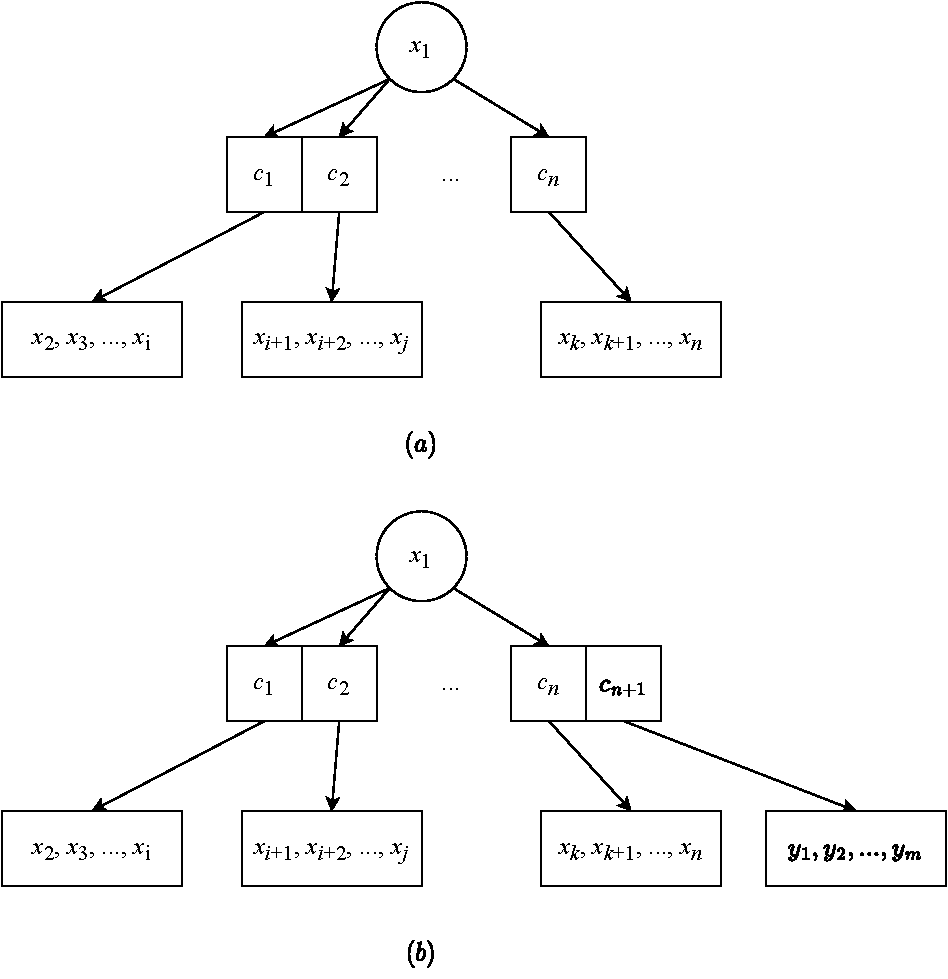
\includegraphics[scale=0.5]{img/clist}} \\
  \subcaptionbox{连接$(y_1, Q_y) = [y_1, y_2, ..., y_m]$相当于入队$c_{n+1}$到$Q_x$}{\includegraphics[scale=0.4]{img/clist1}}
  \caption{可连接列表}
  \label{fig:clist}
\end{figure}

\be
\begin{array}{rcl}
s \doubleplus \nil & = & s \\
\nil \doubleplus s & = & s \\
(x, Q) \doubleplus s & = & (x,\ push\ s\ Q) \\
\end{array}
\ee

插入新元素$z$时,我们先创建一个单元素列表$(z, \nil)$,然后将其连接起来。

\be
\begin{cases}
insert\ x\ s & = (x, \nil) \doubleplus s \\
append\ x\ s & = s \doubleplus (x, \nil) \\
\end{cases}
\ee

从可连接列表的头部删除元素需要单独的设计。$x_1$为根节点,删除后剩下的所有子树也都是由多叉树表示的可连接列表。我们可以把它们全部连接到一起,形成一个新列表。

\be
\begin{array}{rcl}
concat\ \nil & = & \nil \\
concat\ Q & = & (top\ Q) \doubleplus concat\ (pop\ Q) \\
\end{array}
\ee

全部子树存储在实时队列中。我们将第一棵子树$c_1$出队,然后递归地将剩余的子树连接在一起成为$s$,最后把$c_1$、$s$连接起来。我们使用$concat$从头部删除元素。

\be
tail\ (x, Q) = concat\ Q
\ee

算法$concat$遍历了队列,逐步归并到一个最终的结果。这本质上相当于对$Q$进行叠加操作\cite{learn-haskell}。

\be
\begin{array}{rcl}
fold\ f\ z\ \nil & = & z \\
fold\ f\ z\ Q & = & f\ (top\ Q)\ (fold\ f\ z\ (pop\ Q)) \\
\end{array}
\ee

其中$f$是用于归并的二元函数,$z$是零元。下面是一些队列叠加的例子,令$Q = [1, 2, ..., 5]$。

\[
\begin{array}{rcl}
fold\ (+)\ 0\ Q & = & 1 + (2 + (3 + (4 + (5 + 0)))) = 15 \\
fold\ (\times)\ 1\ Q\ & = & 1 \times (2 \times (3 \times (4 \times (5 \times 1)))) = 120 \\
fold\ (\times)\ 0\ Q & = & 1 \times (2 \times (3 \times (4 \times (5 \times 0)))) = 0 \\
\end{array}
\]

我们可以利用叠加来定义$concat$(克里化形式):

\be
concat = fold\ (\doubleplus)\ \nil
\ee

删除操作的性能在最坏情况下是线性的。当连续向空序列添加$n$个元素后,立即执行一次删除。此时多叉树中的$n-1$棵子树都是单元素的(只含有一个叶子节点)。$concat$需要$O(n)$时间进行归并。如果插入、添加、删除、连接随机发生,则分摊复杂度是常数时间的。

\begin{Exercise}
\Question{证明可连接列表的删除操作的分摊复杂度为常数时间的。} %Banker方法
\end{Exercise}

\section{手指树}
\index{序列!手指树}

二叉随机访问列表可以在头部用常数时间(分摊)插入、删除,以对数时间进行随机访问。但是难以向尾部添加元素、也无法进行快速连接。可连接列表能够用常数时间(分摊)进行连接,在头、尾部用常数时间插入。但不能用索引进行随机访问。这两个例子提示我们:1、需要某种方式快速访问头、尾以进行增删;2、带有递归的结构(例如树)可将随机访问转换成分而治之的搜索。手指树\cite{finger-tree-1977}利用了这两点来实现序列\cite{finger-tree-2006}。树是否平衡对搜索性能至关重要。手指树利用了2-3树(一种B-树)。一棵2-3树包含二或三棵子树,如:$(t_1, t_2)$或$(t_1, t_2, t_3)$。

\lstset{frame = single}
\begin{Haskell}
data Node a = Br2 a a | Br3 a a a
\end{Haskell}

我们定义一棵手指树为:

\begin{enumerate}
\item 或者为空$\nil$;
\item 或者是单元素叶子$(x)$;
\item 或者包含三部分:一棵子树和左、右手指,记为$(f, t, r)$。每个手指是一个至多3个元素的列表\footnote{分别是英文前(front)、后(rear)的首字母。}。
\end{enumerate}

\begin{Haskell}
data Tree a = Empty
            | Lf a
            | Tr [a] (Tree (Node a)) [a]
\end{Haskell}

\subsection{插入}

\begin{figure}[htbp]
  \centering
  \subcaptionbox{$\nil$}{\hspace{0.2\textwidth}\includegraphics[scale=0.5]{img/ftr-empty}\hspace{0.2\textwidth}}
  \subcaptionbox{$(x)$}{\hspace{0.2\textwidth}\includegraphics[scale=0.5]{img/ftr-leaf}\hspace{0.2\textwidth}} \\
  \subcaptionbox{$([b], \nil, [a])$}{\includegraphics[scale=0.5]{img/ftr-ab}}
  \caption{手指树,例1}
  \label{fig:ftr-example-1}
\end{figure}

\begin{figure}[htbp]
  \centering
  \subcaptionbox{向$f$手指插入3个元素后,超过了2-3树的限制,不再平衡。}{\includegraphics[scale=0.5]{img/ftr-abcde}}
  \hspace{0.2\textwidth}
  \subcaptionbox{恢复平衡。$f$手指含有2个元素;中间部分为叶子,包含一棵2-3树。}{\includegraphics[scale=0.5]{img/ftr-abcdef}}
  \caption{手指树,例2}
\label{fig:ftr-example-2}
\end{figure}

如图\ref{fig:ftr-example-1}和\ref{fig:ftr-example-2}所示。例1中(a)为$\nil$,(b)是插入一个元素后的结果。(c)含有两个元素,分别在$f$、$r$手指中。如果继续插入元素,$f$手指会超过2-3树的限制,如例2(a)所示。(b)恢复平衡后,$f$手指中有2个元素,中间部分是一个含有一棵2-3树的叶子。这些例子可以表示为:

\[
\begin{array}{ll}
\nil & \texttt{Empty}\\
(a) & \texttt{Lf a}\\
([b], \nil, [a]) & \texttt{Tr [b] Empty [a]}\\
([e, d, c, b], \nil, [a]) & \texttt{Tr [e, d, c, b] Empty [a]}\\
([f, e], (d, c, b), [a]) & \texttt{Tr [f, e] Lf (Br3 d c b) [a]}\\
\end{array}
\]

\index{手指树!头部插入}
注意最后一个例子中,中间部分的子树是一个叶子。手指树是递归的。除去$f$、$r$手指的中间部分是一棵更深的手指树,定义为$Tree\ (Node\ a)$。深度增加一级,就多嵌套一级。上面的例子实际描述了向手指树插入元素的过程。我们可以归纳如下。向一棵手指树$T$中插入$a$时:

\begin{enumerate}
\item 如果$T = \nil$,则结果为单元素叶子$(a)$;
\item 如果$T = (b)$是一个叶子,结果为$([a], \nil, [b])$;
\item $T = (f, t, r)$,如果$f$中元素个数不超过3,将$a$插入到$f$中,如果$f$中元素个数超过3。将$f$中的后3个元素移入一棵新的2-3树$t'$,递归地将$t'$插入到$t$中。最后将$a$插入到$f$中。
\end{enumerate}

\be
\begin{array}{rcl}
insert\ a\ \nil & = & (x) \\
insert\ a\ (b) & = & ([a], \nil, [b]) \\
insert\ a\ ([b, c, d, e], t, r) & = & ([a, b], insert\ (c, d, e)\ t, r) \\
insert\ a\ (f, t, r) & = & (a \cons f, t, r) \\
\end{array}
\ee

除了递归插入外,其它情况插入都需要常数时间。递归深度取决于树的高度$h$,由于使用2-3树并维持平衡,因此$h= O(\lg n)$,其中$n$是手指树中存储元素的个数。递归可以分摊到其它情况中,插入的分摊复杂度为常数时间\cite{okasaki-book}\cite{finger-tree-2006}。我们可以利用叠加连续将若干元素插入到树中:

\be
xs \gg t = foldr\ insert\ t\ xs
\ee

\begin{Exercise}
\Question{消除递归,用循环的方式实现手指树插入。}
\end{Exercise}

\begin{Answer}
\Question{消除递归,用循环的方式实现手指树插入。
对于手指树$T = (f, t, r)$,令$\textproc{Mid}(T) = t$以获取中间部分。

\begin{algorithmic}[1]
\Function{Insert}{$x, T$}
  \State $n = (x)$
  \State $\perp \gets p \gets ([\ ], T, [\ ])$
  \While{$|\textproc{Front}(T)| \geq 3$}
    \State $f \gets \textproc{Front}(T)$
    \State $n \gets (f[2], f[3], ...)$
    \State $\textproc{Front}(T) \gets [n, f[1]]$
    \State $p \gets T$
    \State $T \gets$ \Call{Mid}{$T$}
  \EndWhile
  \If{$T =$ NIL}
    \State $T \gets ([n], \text{NIL}, [\ ])$
  \ElsIf{ $|\textproc{Front}(T)| = 1$ and $\textproc{Rear}(T) = [\ ]$}
    \State \Call{Rear}{$T$} $\gets$ \Call{Front}{$T$}
    \State \Call{Front}{$T$} $\gets [n]$
  \Else
    \State \textproc{Insert}(\Call{Front}{$T$}, $n$)
  \EndIf
  \State \Call{Mid}{$p$} $\gets T$
  \State $T \gets$ \Call{Mid}{$\perp$}, \Call{Mid}{$\perp$} $\gets$ NIL
  \State \Return $T$
\EndFunction
\end{algorithmic}

我们将待插入元素$x$装入一个单元素叶子$(x)$。如果$f$手指超出3个元素,就沿着中间子树,进行一次自顶向下的遍历。我们将$f$中除第一个元素外的剩余部分抽出,放入一个新节点$n$(深度增加1),然后继续将$n$插入到中间子树中。将待插入内容和$f$中剩下的一个元素组成新的$f$手指。遍历结束后,我们要么到达了一个空树,要么到达了一棵子树,这棵子树的$f$手指仍可容纳更多元素。对于第一种情况,我们创建一个叶子节点,对于后一种情况,我们将$n$插入到$f$最前面。最后,我们返回树的根$T$。为了简化处理,我们创建了一个特殊的$\perp$节点,它是根节点的父节点。
}
\end{Answer}

\subsection{删除}
\index{手指树!头部删除}

从头部删除可以看作对\textit{insert}进行逆操作。

\be
\begin{array}{rcl}
extract\ (a) & = & (a, \nil) \\
extract\ ([a], \nil, [b]) & = & (a, (b)) \\
extract\ ([a], \nil, b \cons bs) & = & (a, ([b], \nil, bs)) \\
extract\ ([a], t, r) & = & (a, (toList\ f, t', r)), \text{其中}: (f, t') = extract\ t \\
extract\ (a \cons as, t, r) & = & (a, (as, t, r)) \\
\end{array}
\ee

其中$toList$将一棵2-3树转换为列表:

\be
\begin{array}{rcl}
toList\ (a, b) & = & [a, b] \\
toList\ (a, b, c) & = & [a, b, c] \\
\end{array}
\ee

我们略过了错误情况(如从空树中删除)。如果手指树是单元素叶子,结果为空树;如果手指树只包含两个元素,我们删除$f$中的元素,结果为单元素的叶子;如果$f$中只含有一个元素,中间部分为空,而$r$不空,我们删除$f$中的唯一元素,然后从$r$中“借”一个元素放入$f$;如果$f$只有一个元素,而中间子树不空,我们就递归地从子树中删除一个节点,然后将这一节点中的内容转换成列表来代替$f$。而原来$f$中的唯一元素被删除;如果$f$包含一个以上的元素,我们将第一个元素删除。图\ref{fig:ftr-uncons-example}展示了从序列头部删除两个元素的例子。

\begin{figure}[htbp]
  \centering
  \subcaptionbox{含有10个元素的树。}{\includegraphics[scale=0.4]{img/ftr-10}} \\
  \subcaptionbox{删除一个元素后,$f$还剩一个元素。}{\includegraphics[scale=0.4]{img/ftr-9}} \\
  \subcaptionbox{再次删除一个元素,从中间子树“借”一个节点,将它从2-3树转换成列表,作为新的$f$。}{\hspace{0.2\textwidth}\includegraphics[scale=0.4]{img/ftr-8}\hspace{0.2\textwidth}}
  \caption{删除}
  \label{fig:ftr-uncons-example}
\end{figure}

使用$extract$,我们可以定义出$head$和$tail$:

\be
\begin{cases}
head & = fst \circ extract \\
tail & = snd \circ extract \\
\end{cases}
\ee

\begin{Exercise}
\Question{消除递归,用循环实现删除。}
\end{Exercise}

\begin{Answer}
\Question{消除递归,用循环实现删除。

如果删除后front手指变空,就从中间部分的子树中“借”节点。但是树的形式有可能是不规则的,例如front手指和中间子树都为空。这种情况通常是由于分拆操作造成的。

\begin{center}
  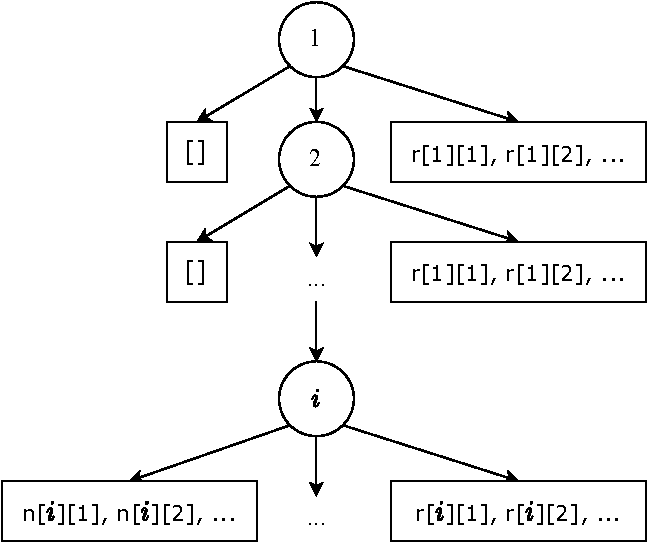
\includegraphics[scale=0.4]{img/ftr-illed-1}
  \captionof{figure}{不规则树,第$i$层子树的$f$不空}
  \label{fig:ftr-illed-form}
\end{center}

我们要从不规则的手指树中删除第一个元素。首先进行一轮自顶向下的遍历,找到一棵子树,或者它的$f$不为空,或者$f$和中间子树都为空,如图\ref{fig:ftr-illed-form}。对于前者,我们可以从$f$中提取出第一个元素(是一个节点)。对于后者,由于只有$r$不为空,我们交换$f$、$r$,转换成前一种情况。此后,我们检查从$f$中取出的节点是否为叶子。如果不是,我们需要继续提取。我们沿着父节点一直向上回溯,直到我们提取到一个叶子节点。此时我们将到达树的根节点。图\ref{fig:ftr-illed-extract}描述了这一过程。

\begin{center}
  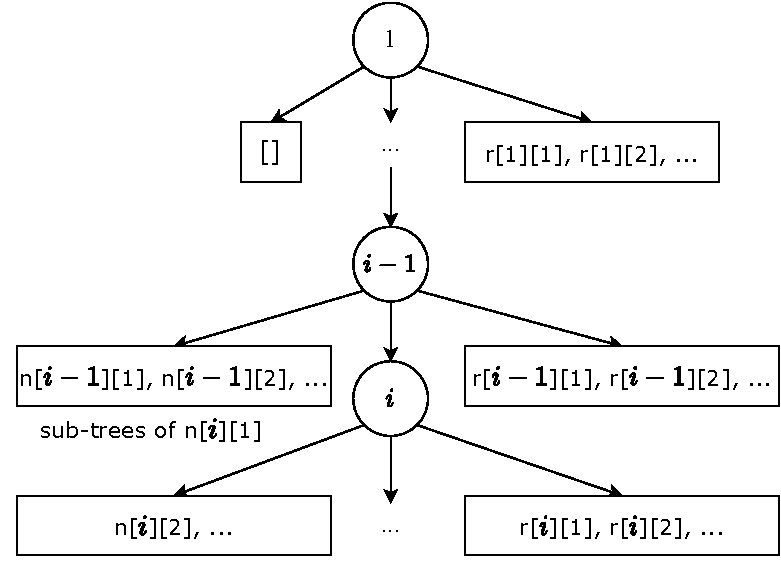
\includegraphics[scale=0.4]{img/ftr-illed-2} \\
  提取第一个元素$n[i][1]$,然后将它的子节点放到上一级树的$f$手指中。\\
  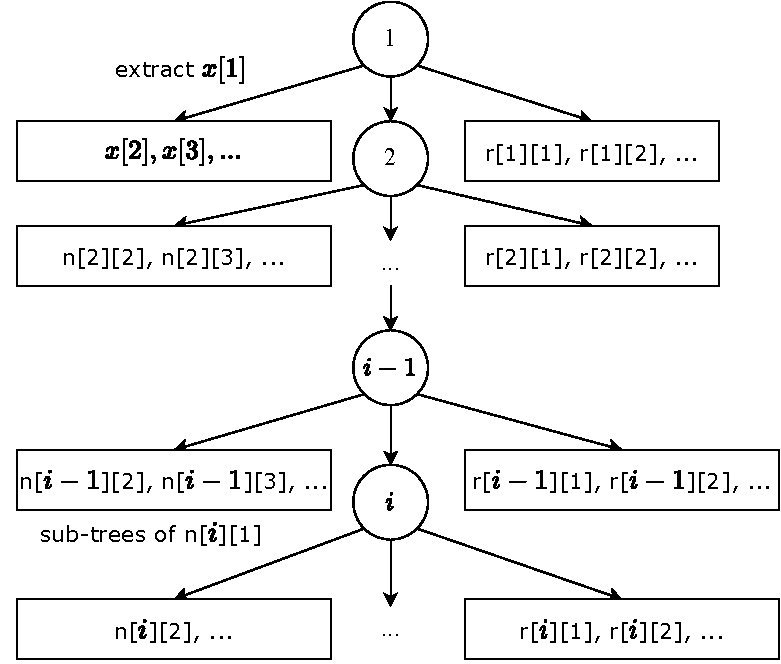
\includegraphics[scale=0.4]{img/ftr-illed-i} \\
  重复$i$次,最终提取到$x[1]$。\\
  \captionof{figure}{自底向上遍历,直到提取出一个叶子节点}
  \label{fig:ftr-illed-extract}
\end{center}

根据这一思路,下面的算法实现了列表头部的删除操作(假设树不为空)。

\begin{algorithmic}[1]
\Function{Extract}{$T$}
  \State $\perp \gets ([], T, [])$
  \While{\Call{Front}{$T$} $= [\ ]$ and \Call{Mid}{$T$} $\neq $ NIL}
    \State $T \gets$ \Call{Mid}{$T$}
  \EndWhile

  \If{\Call{Front}{$T$} $ = [\ ]$ and \Call{Rear}{$T$} $\neq [\ ]$}
    \State \textproc{Exchange} \Call{Front}{$T$} $\leftrightarrow$ \Call{Rear}{$T$}
  \EndIf

  \State $f \gets$ \Call{Front}{$T$}, $r \gets$ \Call{Rear}{$T$}
  \State $n \gets (f[1], f[2], ...)$ \Comment{$n$是2-3树}
  \Repeat
    \State \Call{Front}{$T$} $\gets [n_2, n_3, ..]$
    \State $n \gets n_1$
    \State $T \gets $ \Call{Parent}{$T$}
    \If{\Call{Mid}{$T$} becomes empty}
      \State \Call{Mid}{$T$} $\gets$ NIL
    \EndIf
  \Until{$n$ is leaf}
  \State \Return (\Call{Elem}{$n$}, \Call{Mid}{$\perp$})
\EndFunction
\end{algorithmic}

这里函数\textproc{Elem}($n$)返回叶子节点$n$中保存的唯一元素。由于不规则的树存在,需要调整从手指树中获取第一个和最后一个元素的定义。我们不再仅返回手指的第一个或者最后一个子节点。如果手指为空,而中间子树不为空,我们就沿着中间部分向下遍历,直到发现手指不为空,或者所有的节点都存储在另一侧的手指中。

\begin{algorithmic}[1]
\Function{First-Leaf}{$T$}
  \While{\Call{Front}{$T$} $ = [\ ]$ and \Call{Mid}{$T$} $\neq$ NIL}
    \State $T \gets$ \Call{Mid}{$T$}
  \EndWhile
  \If{\Call{Front}{$T$} $ = [\ ]$ and \Call{Rear}{$T$} $\neq [\ ]$}
    \State $n \gets$ \Call{Rear}{$T$}[1]
  \Else
    \State $n \gets$ \Call{Front}{$T$}[1]
  \EndIf
  \While{$n$ is NOT leaf}
    \State $n \gets n_1$
  \EndWhile
  \State \Return $n$
\EndFunction
\Statex
\Function{First}{$T$}
  \State \Return \textproc{Elem}(\Call{First-Leaf}{$T$})
\EndFunction
\end{algorithmic}

其中第二个循环中,如果节点不是叶子,就不断沿着第一个子节点遍历。获取最后一个元素与此类似.
}
\end{Answer}

\subsection{尾部操作}
\index{手指树!尾部添加}

我们可以对称地实现尾部添加、删除。

\be
\begin{array}{rcl}
append\ \nil\ a & = & (a) \\
append\ (a)\ b & = & ([a], \nil, [b]) \\
append\ (f, t, [a, b, c, d])\ e & = & (f, append\ t\ (a, b, c), [d, e]) \\
append\ (f, t, r)\ a & = & (f, t, r \doubleplus [a]) \\
\end{array}
\ee

如果$r$中的元素不超过4个,仍是合法的2-3树,我们直接把新元素添加到$r$末尾。否则,将$r$中的前三个元素取出,构造一棵新的2-3树,递归地添加到中间子树的尾部。类似地我们可以用左侧叠加连续将若干元素构造成一棵手指树:

\be
t \ll xs = foldl\ append\ t\ xs
\ee

\index{手指树!尾部删除}
从尾部删除相当于添加的逆操作:

\be
\begin{array}{rcl}
remove\ (a) & = & (\nil, a) \\
remove\ ([a], \nil, [b]) & = & ((a), b) \\
remove\ (f, \nil, [a]) & = & ((init f, \nil, [last f]), a) \\
remove\ (f, t, [a]) & = & ((f, t', toList\ r), a), \text{其中}: (t', r) = remove\ t \\
remove\ (f, t, r) & = & ((f, t, init\ r), last\ r) \\
\end{array}
\ee

其中$last$获取列表的最后一个元素,$init$返回其余部分(定义见第一章)。

\subsection{连接}
\index{手指树!连接}

考虑两棵手指树都不为空的情况:$T_1 = (f_1, t_1, r_1)$、$T_2 = (f_2, t_2, r_2)$。我们用$f_1$作为连接结果中的$f$,用$r_2$作为结果中的$r$。然后将$t_1$、$r_1$、$f_2$、$t_2$合并成中间子树。由于$r_1$和$f_2$都是节点的列表,所以这等价于如下问题:

\[
merge\ t_1\ (r_1 \doubleplus f_2)\ t_2 = ?
\]

$t_1$和$t_2$也都是手指树,但它们比$T_1$和$T_2$深一级,若$T_1$中的元素类型为$a$,则$t_1$中的元素类型为$Node\ a$。我们递归地进行合并:保留$t_1$的$f$手指和$t_2$的$r$手指,然后将$t_1$和$t_2$的中间部分,$t_1$的$r$手指和$t_2$的$f$手指合并。

\be
\begin{array}{rcl}
merge\ \nil\ ts\ t_2 & = & ts \gg t_2 \\
merge\ t_1\ ts\ \nil & = & t_1 \ll ts \\
merge\ (a)\ ts\ t_2 & = & merge\ \nil\ (a \cons ts)\ t_2 \\
merge\ t_1\ ts\ (a) & = & merge\ t_1\ (ts \doubleplus [a])\ \nil \\
merge\ (f_1, t_1, r_1)\ ts\ (f_2, t_2, r_2) & = & (f_1, merge\ t_1\ (nodes\ (r_1 \doubleplus ts \doubleplus f_2))\ t_2, r_2) \\
\end{array}
\label{eq:merge-recursion}
\ee

其中$nodes$将若干元素组织成一组2-3树。这是因为中间子树中的元素类型,比手指中的元素类深一级。

\be
\begin{array}{rcl}
nodes\ [a, b] & = & [(a, b)] \\
nodes\ [a, b, c] & = & [(a, b, c)] \\
nodes\ [a, b, c, d] & = & [(a, b), (c, d)] \\
nodes\ (a \cons b \cons c \cons ts) & = & (a, b, c) \cons nodes\ ts \\
\end{array}
\ee

这样我们可以用$merge$来定义手指树的连接:

\be
(f_1, t_1, r_1) \doubleplus (f_2, t_2, r_2) = (f_1, merge\ t_1\ (r_1 \doubleplus f_2)\ t_2, r_2)
\ee

比较这一定义和(\ref{eq:merge-recursion}),连接操作本质上就是合并操作,我们可以给出下面更加一致的定义:

\be
T_1 \doubleplus T_2 = merge\ T_1\ [\ ]\ T_2
\ee

连接的性能取决于递归的合并操作。递归的深度为两棵树中较小的一棵。由于2-3树的平衡性,手指树的高度为$O(\lg n)$其中$n$为元素的个数。合并在边界条件下的性能和插入一样(最多调用$insert$\ 8次)为分摊常数时间,最坏情况为$O(\lg m)$,其中$m$是两棵树的高度差。总体上算法的复杂度为$O(\lg n)$,其中$n$是两棵手指树中含有的元素总数。

\subsection{随机访问}
\index{手指树!随机访问}

我们的策略是把随机访问转换为树搜索。为了避免反复计算树的大小,我们给每个节点增加一个$s$变量记录其包含的元素个数:$(s, f, t, r)$。

\begin{Haskell}
data Tree a = Empty
            | Lf a
            | Tr Int [a] (Tree (Node a)) [a]
\end{Haskell}

\be
\begin{array}{rcl}
size\ \nil & = & 0 \\
size\ (x) & = & size\ x \\
size\ (s, f, t, r) & = & s \\
\end{array}
\ee

这里$size\ (x)$并不一定是1。这是因为$x$可能是更深的节点,例如$Node\ a$,而只有当第一层时大小才是1。为此我们可以在插入或添加时,把每个元素$x$包装在一个单元里$(x)_e$,规定这个单元的大小为1,即:$size\ (x)_e = 1$(参见附录例子)。

\be
\begin{cases}
x \lhd t = insert\ (x)_e\ t \\
t \rhd x = append\ t\ (x)_e \\
\end{cases}
\ee

以及:
\be
\begin{cases}
xs \ll t = foldr\ (\lhd)\ t\ xs \\
t \gg xs = foldl\ (\rhd)\ t\ xs \\
\end{cases}
\ee

我们还需要获取2-3树的大小:

\be
\begin{array}{rcl}
size\ (t_1, t_2) & = & size\ t_1 + size\ t_2 \\
size\ (t_1, t_2, t_3) & = & size\ t_1 + size\ t_2 + size\ t_3 \\
\end{array}
\ee

\index{手指树!随机访问}
对于节点的列表(例如深一级的手指)我们可以用$sum \circ (map\ size)$来计算大小。在插入和删除操作中,我们也需要更新树大小。增加大小信息后,给定一个位置$i$,可以通过树搜索定位到相应的节点。手指树具有递归结构:$(s, f, t, r)$,我们令这些子结构的大小为:$s_f$、$s_t$、$s_r$,且$s = s_f + s_t + s_r$。如果$i \leq s_f$,则目标位于$f$中,我们接下来在$f$中查找;如果$s_f < i \leq s_f + s_t$,则目标位于$t$中,我们递归在$t$中搜索;否则目标位于$r$中。除此之外,我们还需要处理叶子节点$(x)$的情况。我们用一对值$(i, t)$表示在数据结构$t$中$i$的位置,并定义查找操作$lookup_T$如下:

\be
\begin{array}{rcl}
lookup_T\ i\ (x) & = & (i, x) \\
lookup_T\ i\ (s, f, t, r) & = & \begin{cases}
  i < s_f: & lookup_s\ i\ f \\
  s_f \leq i < s_f + s_t: & lookup_N\ (lookup_T\ (i - s_f)\ t) \\
  \text{否则}: & lookup_s\ (i - s_f - s_t)\ r \\
\end{cases}
\end{array}
\ee

这里:$s_f = sum\ (map\ size\ f), s_t = size\ t$,分别是手指树前两部分的大小。如果在叶子节点$(x)$中查找位于$i$的内容,结果为$(i, x)$。否则我们判断$i$位于$(s, f, t, r)$中哪一部分。如果位于前后手指$f, r$中,我们依次查找手指列表中的每个元素。

\be
\begin{array}{rcl}
lookup_s\ i\ (x \cons xs) = \begin{cases}
  i < size\ x: & (i, x) \\
  \text{否则}: & lookup_s\ (i - size\ x)\ xs \\
\end{cases}
\end{array}
\ee

如果$i$位于某个元素$x$中($i < size\ x$),我们返回$(i, x)$,否则我们继续查找后面的元素。如果$i$不位于前后手指$f, r$,而在中间部分$t$,我们递归地在更深层查找,得到位置$(i', m)$。这里$m$是一个2-3树,我们接下来在其中查找:

\be
\begin{array}{rcl}
lookup_N\ i\ (t_1, t_2) & = & \begin{cases}
  i < size\ t_1: & (i, t_1) \\
  \text{否则}: & (i - size\ t_1, t_2) \\
\end{cases} \\
lookup_N\ i\ (t_1, t_2, t_3) & = & \begin{cases}
  i < size\ t_1: & (i, t_1) \\
  size\ t_1 \leq i < size\ t_1 + size\ t_2: & (i - size\ t_1, t_2) \\
  \text{否则}: & (i - size\ t_1 - size\ t_2, t_3) \\
\end{cases} \\
\end{array}
\ee

我们此前为了计算大小把每个元素$x$都封装在$(x)_e$中,最终我们需要从中把$x$取回:

\be
T[i] = \begin{cases}
  \text{若} lookup_T\ i\ T = (i', (x)_e): & \textit{Just}\ x \\
  \text{否则}: & \textit{Nothing}
\end{cases}
\ee

我们利用了类型$\textit{Maybe}\ a = \textit{Nothing} | \textit{Just}\ a$来表示索引成功或没有找到\footnote{很多编程环境提供了类似的处理,例如Java/C++中的\texttt{Optional<T>}类型}。随机访问需要递归在手指树中查找,递归次数取决于树的深度。由于手指树是平衡的,随机访问的复杂度为$O(\lg n)$,其中$n$是存储的元素个数。

\index{MTF}
我们用手指树实现的序列在总体上有着均衡、良好的性能。头、尾操作的分摊复杂度为常数时间,可以在对数时间内进行连接、分割、随机索引\cite{hackage-ftr}。到本章为止,我们介绍了最基本的数据结构。接下来可以使用它们解决一些典型问题。例如,我们可以用序列实现实现MTF\footnote{英文move to front的缩写。它应用于BWT (Burrows-Wheeler transform)数据压缩算法。}编码算法\cite{mtf-wiki}。MTF把序列中任意位置$i$的元素移动到最前面:

\[
mtf\ i\ S = x \lhd S', \text{其中}(x, S') = \textit{extractAt}\ i\ S
\]

在后面章节中,我们将介绍基本的分而治之的排序算法,包括快速排序、归并排序以及它们的变形;然后我们介绍字符串匹配算法和基本搜索算法。

\begin{Exercise}
\Question{在随机访问时,如何处理空树$\nil$和索引越界的情况?}
\Question{实现$cut\ i\ S$,在位置$i$把序列$S$分割开。}
\end{Exercise}

\begin{Answer}
\Question{在随机访问时,如何处理空树$\nil$和索引越界的情况?

我们可以在索引时进行越界检查,例如:
\[
\begin{array}{rcl}
\nil [i] & = & \textit{Nothing} \\
T [i] & = & \begin{cases}
  i < 0\ \text{或}\ i \geq size\ T: & \textit{Nothing} \\
  \text{否则}: & ...
\end{cases}
\end{array}
\]
}
\Question{实现$cut\ i\ S$,在位置$i$把序列$S$分割开。

我们给出一种手指树分割的实现(手指树的基本定义参考本章的附录例子)。我们首先进行基本的越界检查,如果$0 \leq i < size\ s$ 我们接下来调用$cutTree\ i\ S$进行分割。

\begin{Haskell}
cut :: Int -> Seq a -> (Seq a, Maybe a, Seq a)
cut i (Seq xs) | i < 0 = (Seq Empty, Nothing, Seq xs)
               | i < size xs = case cutTree i xs of
                 (a, Just (Place _ (Elem x)), b) -> (Seq a, Just x, Seq b)
                 (a, Nothing, b) -> (Seq a, Nothing, Seq b)
               | otherwise = (Seq xs, Nothing, Seq Empty)
\end{Haskell}

\textit{cutTree}把树分割成三部分:左侧、中间、右侧。中间部分利用\textit{Maybe}类型表示可能查找不到。如果找到则包含需要进一步索引的位置$i'$和节点$a$,封装在一个\textit{Place}类型中。如果索引$i$位于前后手指$f, r$中,我们调用$cutList$进一步分割,并将分割后的结果组装起来;如果$i$位于中间,则递归分割。然后对结果$\textit{Place}\ i'\ a$中的2-3树$a$在位置$i'$进一步分割。

\begin{Haskell}
cutTree :: (Sized a) => Int -> Tree a -> (Tree a, Maybe (Place a), Tree a)
cutTree _ Empty = (Empty, Nothing, Empty)
cutTree i (Lf a) | i < size a = (Empty, Just (Place i a), Empty)
                 | otherwise = (Lf a, Nothing, Empty)
cutTree i (Br s f m r)
  | i < sf = case cutList i f of
               (xs, x, ys) -> (Empty <<< xs, x, tree ys m r)
  | i < sm = case cutTree (i - sf) m of
               (t1, Just (Place i' a), t2) -> let (xs, x, ys) = cutNode i' a
                 in (tree f t1 xs, x, tree ys t2 r)
  | i < s  = case cutList (i - sm) r of
               (xs, x, ys) -> (tree f m xs, x, ys >>> Empty)
  where
    sf = sum $ map size f
    sm = sf + size m
\end{Haskell}

其中$tree\ f\ m\ r$构造出一个手指树,并进行适当的化简:

\begin{Haskell}
tree as Empty [] = as >>> Empty
tree [] Empty bs = Empty <<< bs
tree [] m r = Br (size m + sum (map size r)) (nodesOf f) m' r
    where (f, m') = uncons m
tree f m [] = Br (size m + sum (map size f)) f m' (nodesOf r)
    where (m', r) = unsnoc m
tree f m r = Br (size m + sum (map size f) + sum (map size r)) f m r
\end{Haskell}

对于手指和2-3树的分割实现如下:

\begin{Haskell}
cutList :: (Sized a) => Int -> [a] -> ([a], Maybe (Place a), [a])
cutList _ [] = ([], Nothing, [])
cutList i (x:xs) | i < sx = ([], Just (Place i x), xs)
                 | otherwise = let (xs', y, ys) = cutList (i - sx) xs
                               in (x:xs', y, ys)
  where sx = size x

cutNode :: (Sized a) => Int -> Node a -> ([a], Maybe (Place a), [a])
cutNode i (Tr2 _ a b) | i < sa = ([], Just (Place i a), [b])
                      | otherwise = ([a], Just (Place (i - sa) b), [])
  where sa = size a
cutNode i (Tr3 _ a b c) | i < sa = ([], Just (Place i a), [b, c])
                        | i < sab = ([a], Just (Place (i - sa) b), [c])
                        | otherwise = ([a, b], Just (Place (i - sab) c), [])
  where sa = size a
        sab = sa + size b
\end{Haskell}

我们可以用分割修改指定位置的元素、删除指定位置的元素、以及MTF操作,它们的复杂度都是$O(\lg n)$。

\begin{Haskell}
setAt s i x = case cut i s of
  (_, Nothing, _) -> s
  (xs, Just y, ys) -> xs +++ (x <| ys)

extractAt s i = case cut i s of (xs, Just y, ys) -> (y, xs +++ ys)

moveToFront i s = if i < 0 || i >= size s then s
                  else let (a, s') = extractAt s i in a <| s'
\end{Haskell}
}
\end{Answer}

\section{附录:例子程序}

随机访问列表(森林):

\lstset{frame = single}
\begin{Haskell}
data Tree a = Leaf a
            | Node Int (Tree a) (Tree a)

type BRAList a = [Tree a]

size (Leaf _) = 1
size (Node sz _ _) = sz

link t1 t2 = Node (size t1 + size t2) t1 t2

insert x = insertTree (Leaf x) where
    insertTree t [] = [t]
    insertTree t (t':ts) = if size t < size t' then  t:t':ts
                           else insertTree (link t t') ts

extract ((Leaf x):ts) = (x, ts)
extract ((Node _ t1 t2):ts) = extract (t1:t2:ts)

head' = fst . extract
tail' = snd . extract

getAt i (t:ts) | i < size t = lookupTree i t
               | otherwise = getAt (i - size t) ts
  where
    lookupTree 0 (Leaf x) = x
    lookupTree i (Node sz t1 t2)
        | i < sz `div` 2 = lookupTree i t1
        | otherwise = lookupTree (i - sz `div` 2) t2
\end{Haskell}

随机访问森林的数值表示:
\begin{Haskell}
data Digit a = Zero | One (Tree a)

type RAList a = [Digit a]

insert x = add (Leaf x) where
  add t [] = [One t]
  add t (Zero:ts) = One t : ts
  add t (One t' :ts) = Zero : add (link t t') ts

minus [One t] = (t, [])
minus (One t:ts) = (t, Zero:ts)
minus (Zero:ts) = (t1, One t2:ts') where
    (Node _ t1 t2, ts') = minus ts

head' ts = x where (Leaf x, _) = minus ts
tail' = snd . minus
\end{Haskell}

双数组序列:

\begin{lstlisting}[language = Bourbaki]
Data Seq<K> {
    [K] front = [], rear = []
}

Int length(S<K> s) = length(s.front) + length(s.rear)

void insert(K x, Seq<K> s) = append(x, s.front)

void append(K x, Seq<K> s) = append(x, s.rear)

K get(Int i, Seq<K> s) {
    Int n = length(s.front)
    return if i < n then s.front[n - i - 1] else s.rear[i - n]
}
\end{lstlisting}

可连接列表:

\begin{Haskell}
data CList a = Empty | CList a (Queue (CList a))

wrap x = CList x emptyQ

x ++ Empty = x
Empty ++ y = y
(CList x q) ++ y = CList x (push q y)

fold f z q | isEmpty q = z
           | otherwise = (top q) `f` fold f z (pop q)

concat = fold (++) Empty

insert x xs = (wrap x) ++ xs
append xs x = xs ++ wrap x

head (CList x _) = x
tail (CList _ q) = concat q
\end{Haskell}

手指树:

\begin{Haskell}
-- 2-3树
data Node a = Tr2 Int a a
            | Tr3 Int a a a

-- 手指树
data Tree a = Empty
            | Lf a
            | Br Int [a] (Tree (Node a)) [a] -- size, front, mid, rear

newtype Elem a = Elem { getElem :: a } -- 封装元素

newtype Seq a = Seq (Tree (Elem a)) -- 序列

class Sized a where  -- 可计算大小
  size :: a -> Int

instance Sized (Elem a) where
  size _ = 1  -- 元素的大小总为1

instance Sized (Node a) where
  size (Tr2 s _ _) = s
  size (Tr3 s _ _ _) = s

instance Sized a => Sized (Tree a) where
  size Empty = 0
  size (Lf a) = size a
  size (Br s _ _ _) = s

instance Sized (Seq a) where
  size (Seq xs) = size xs

tr2 a b = Tr2 (size a + size b) a b
tr3 a b c = Tr3 (size a + size b + size c) a b c

nodesOf (Tr2 _ a b) = [a, b]
nodesOf (Tr3 _ a b c) = [a, b, c]

-- 左侧操作
x <| Seq xs = Seq (Elem x `cons` xs)

cons :: (Sized a) => a -> Tree a -> Tree a
cons a Empty = Lf a
cons a (Lf b) = Br (size a + size b) [a] Empty [b]
cons a (Br s [b, c, d, e] m r) = Br (s + size a) [a, b] ((tr3 c d e) `cons` m) r
cons a (Br s f m r) = Br (s + size a) (a:f) m r

head' (Seq xs) = getElem $ fst $ uncons xs
tail' (Seq xs) = Seq $ snd $ uncons xs

uncons :: (Sized a) => Tree a -> (a, Tree a)
uncons (Lf a) = (a, Empty)
uncons (Br _ [a] Empty [b]) = (a, Lf b)
uncons (Br s [a] Empty (r:rs)) = (a, Br (s - size a) [r] Empty rs)
uncons (Br s [a] m r) = (a, Br (s - size a) (nodesOf f) m' r)
    where (f, m') = uncons m
uncons (Br s (a:f) m r) = (a, Br (s - size a) f m r)

-- 右侧操作
Seq xs |> x  = Seq (xs `snoc` Elem x)

snoc :: (Sized a) => Tree a -> a -> Tree a
snoc Empty a = Lf a
snoc (Lf a) b = Br (size a + size b) [a] Empty [b]
snoc (Br s f m [a, b, c, d]) e = Br (s + size e) f (m `snoc` (tr3 a b c)) [d, e]
snoc (Br s f m r) a = Br (s + size a) f m (r ++ [a])

last' (Seq xs) = getElem $ snd $ unsnoc xs
init' (Seq xs) = Seq $ fst $ unsnoc xs

unsnoc :: (Sized a) => Tree a -> (Tree a, a)
unsnoc (Lf a) = (Empty, a)
unsnoc (Br _ [a] Empty [b]) = (Lf a, b)
unsnoc (Br s f@(_:_:_) Empty [a]) = (Br (s - size a) (init f) Empty [last f], a)
unsnoc (Br s f m [a]) = (Br (s - size a) f m' (nodesOf r), a)
    where (m', r) = unsnoc m
unsnoc (Br s f m r) = (Br (s - size a) f m (init r), a) where a = last r

-- 连接
Seq xs +++ Seq ys = Seq (xs >+< ys)

xs >+< ys = merge xs [] ys

t <<< xs = foldl snoc t xs
xs >>> t = foldr cons t xs

merge :: (Sized a) => Tree a -> [a] -> Tree a -> Tree a
merge Empty es t2 = es >>> t2
merge t1 es Empty = t1 <<< es
merge (Lf a) es t2 = merge Empty (a:es) t2
merge t1 es (Lf a) = merge t1 (es++[a]) Empty
merge (Br s1 f1 m1 r1) es (Br s2 f2 m2 r2) =
    Br (s1 + s2 + (sum $ map size es)) f1 (merge m1 (trees (r1 ++ es ++ f2)) m2) r2

trees [a, b] = [tr2 a b]
trees [a, b, c] = [tr3 a b c]
trees [a, b, c, d] = [tr2 a b, tr2 c d]
trees (a:b:c:es) = (tr3 a b c):trees es

-- 索引
data Place a = Place Int a

getAt :: Seq a -> Int -> Maybe a
getAt (Seq xs) i | i < size xs = case lookupTree i xs of
                     Place _ (Elem x) -> Just x
                 | otherwise = Nothing

lookupTree :: (Sized a) => Int -> Tree a -> Place a
lookupTree n (Lf a) = Place n a
lookupTree n (Br s f m r) | n < sf = lookups n f
                          | n < sm = case lookupTree (n - sf) m of
                                            Place n' xs -> lookupNode n' xs
                          | n < s = lookups (n - sm) r
  where sf = sum $ map size f
        sm = sf + size m

lookupNode :: (Sized a) => Int -> Node a -> Place a
lookupNode n (Tr2 _ a b) | n < sa = Place n a
                         | otherwise = Place (n - sa) b
  where sa = size a
lookupNode n (Tr3 _ a b c) | n < sa = Place n a
                           | n < sab = Place (n - sa) b
                           | otherwise = Place (n - sab) c
  where sa = size a
        sab = sa + size b

lookups :: (Sized a) => Int -> [a] -> Place a
lookups n (x:xs) = if n < sx then Place n x
                   else lookups (n - sx) xs
  where sx = size x
\end{Haskell}

\ifx\wholebook\relax \else
\section{参考答案}
\shipoutAnswer

\begin{thebibliography}{99}

\bibitem{okasaki-book}
Chris Okasaki. ``Purely Functional Data Structures''. Cambridge university press, (July 1, 1999), ISBN-13: 978-0521663502

\bibitem{okasaki-ralist}
Chris Okasaki. ``Purely Functional Random-Access Lists''. Functional Programming Languages and Computer Architecture, June 1995, pages 86-95.

\bibitem{CLRS}
Thomas H. Cormen, Charles E. Leiserson, Ronald L. Rivest and Clifford Stein. ``Introduction to Algorithms, Second Edition''. The MIT Press, 2001. ISBN: 0262032937.(《算法导论》中文版)

\bibitem{learn-haskell}
Miran Lipovaca. ``Learn You a Haskell for Great Good! A Beginner's Guide''. No Starch Press; 1 edition April 2011, 400 pp. ISBN: 978-1-59327-283-8

\bibitem{finger-tree-2006}
Ralf Hinze and Ross Paterson. ``Finger Trees: A Simple General-purpose Data Structure,'' in Journal of Functional Programming 16:2 (2006), pages 197-217. \url{http://www.soi.city.ac.uk/~ross/papers/FingerTree.html}

\bibitem{finger-tree-1977}
Guibas, L. J., McCreight, E. M., Plass, M. F., Roberts, J. R. (1977), "A new representation for linear lists". Conference Record of the Ninth Annual ACM Symposium on Theory of Computing, pp. 49-60.

\bibitem{hackage-ftr}
Generic finger-tree structure. \url{http://hackage.haskell.org/packages/archive/fingertree/0.0/doc/html/Data-FingerTree.html}

\bibitem{mtf-wiki}
Wikipedia. Move-to-front transform. \url{https://en.wikipedia.org/wiki/Move-to-front_transform}

\end{thebibliography}

\expandafter\enddocument
\fi
